% !TEX program = xelatex
\documentclass[sigconf,nonacm]{acmart}

\usepackage{kotex}
\usepackage{graphicx}
\usepackage{booktabs}
\usepackage{array}
\usepackage{enumitem}
\usepackage{balance}
\setlist[itemize]{leftmargin=*,nosep}
\settopmatter{printacmref=false, printccs=false, printfolios=true}
\renewcommand\footnotetextcopyrightpermission[1]{}
\pagestyle{plain}

\title{GPIoT: IoT 프로그램 합성과 개발을 위해 소형 언어 모델을 맞춤화하기}
\author{Leming Shen, Qiang Yang, Xinyu Huang, Zijing Ma, Yuanqing Zheng}
\affiliation{\institution{SenSys 2025}}
\email{}

\begin{document}
\maketitle

\begin{abstract}
코드 거대 언어 모델(LLM)은 사용자 요구사항으로부터 코드와 문서를 자동 생성해 소프트웨어 개발 효율을 높인다. 하지만 도메인 지식이 필요한 IoT 애플리케이션을 다룰 때, 기존 코드 LLM은 전문화된 프로그램을 합성하지 못한다. 검색 증강 생성(RAG)은 관련 도메인 지식을 가져와 보완하는 방법으로 유망하지만, 사용자 요구사항과 검색 결과를 처리하기 위해 강력한 클라우드 LLM(예: GPT-4)이 필요하므로 프라이버시 우려가 크다. 또한 네트워크 불안정과 비싼 질의 비용 문제도 있으며, 검색된 내용의 정확성과 관련성을 보장하기도 어렵다. 본 논문은 이러한 문제를 해결하기 위해, 로컬에 배포 가능한 소형 언어 모델(SLM)을 IoT 전문 데이터셋으로 파인튜닝하여 IoT 애플리케이션 코드 생성 시스템 GPIoT를 제안한다. SLM은 모델 크기가 작아 로컬 배포와 실행이 효율적이고, 프라이버시와 네트워크 불확실성을 완화한다. 또한 IoT 전문 데이터셋으로 파인튜닝하면 SLM의 IoT 관련 프로그램 합성 능력이 크게 향상된다. GPIoT의 IoT 프로그램 합성 능력을 평가하기 위해 저자들은 벤치마크인 IoTBench도 제안한다. 광범위한 실험과 사용자 평가에서 GPIoT는 최신 코드 LLM 대비 평균 64.7\%의 작업 정확도 향상과 함께 사용자 만족도에서도 큰 개선을 보였다.
\end{abstract}

\begin{figure}[t]
  \centering
  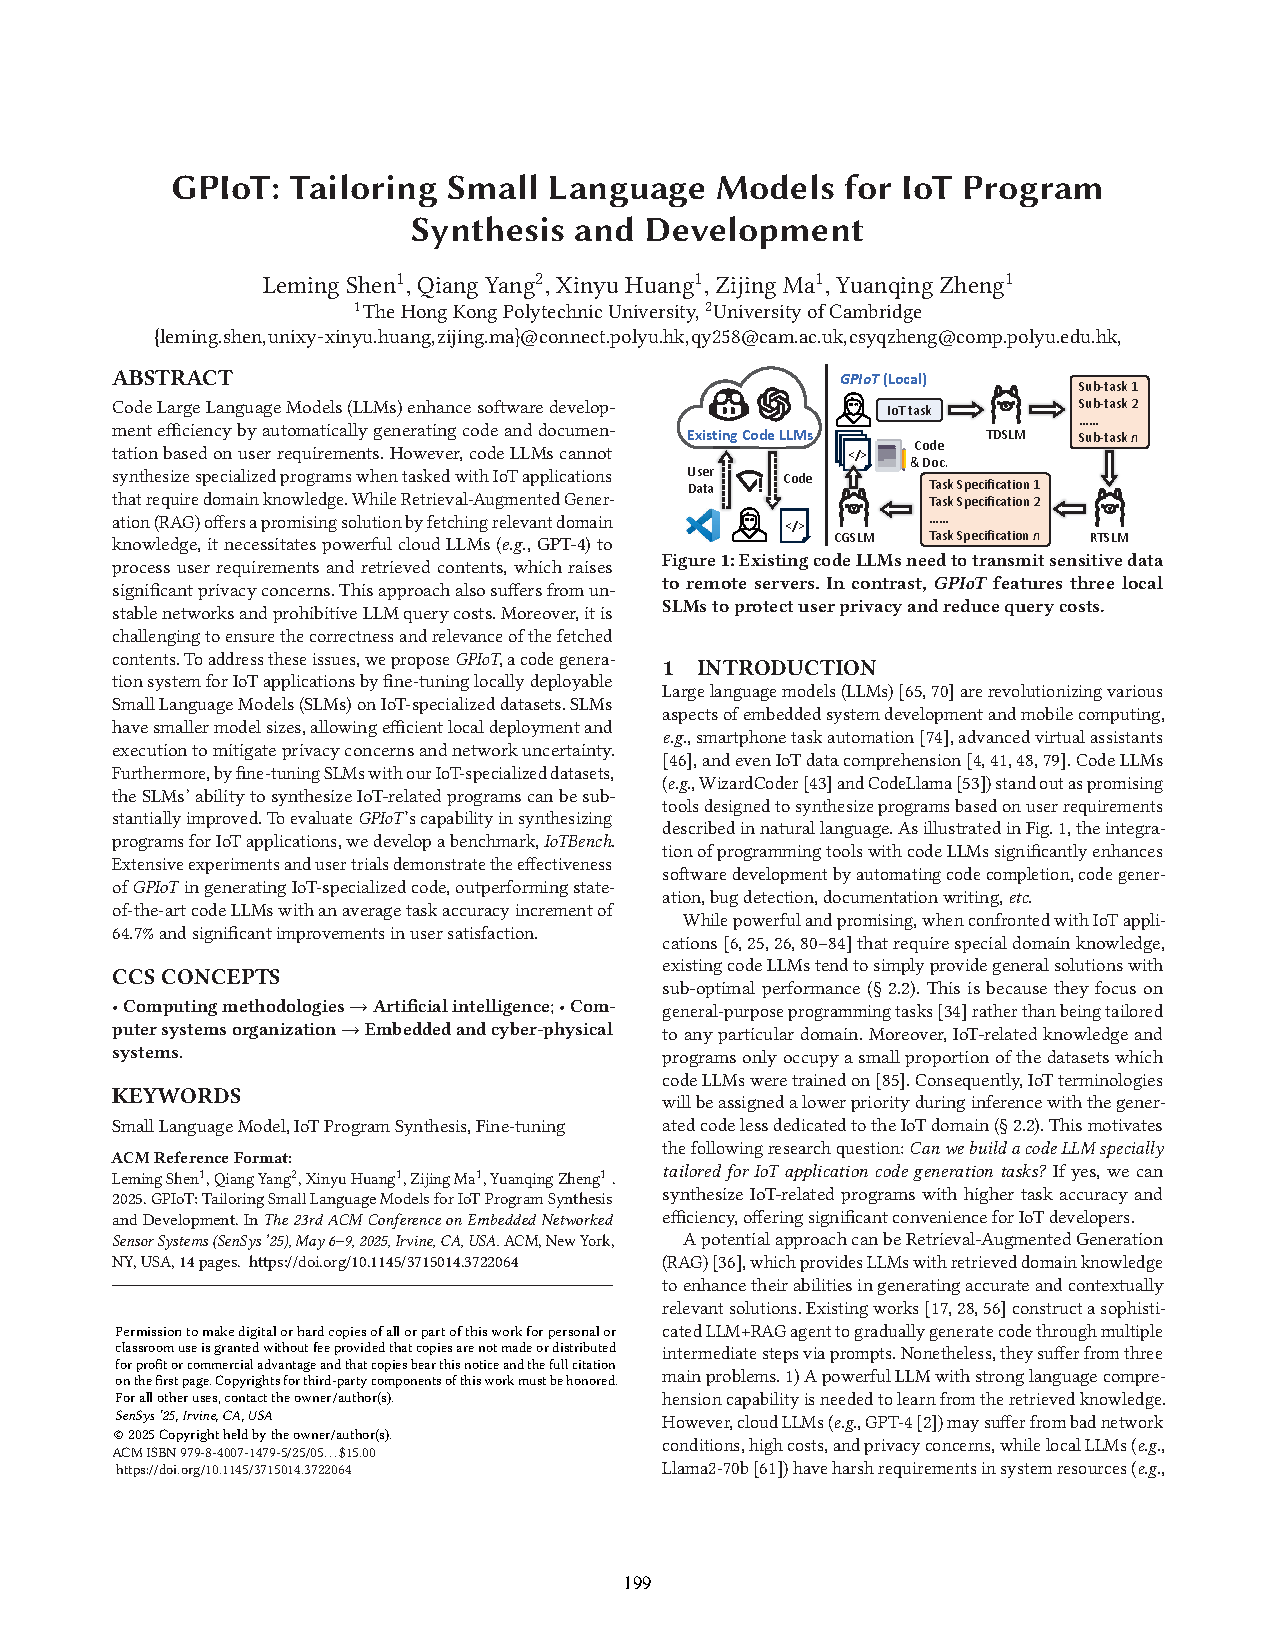
\includegraphics[page=1,width=\columnwidth,trim={317bp 475bp 22bp 130bp},clip]{GPIoT.pdf}
  \caption{Figure 1: Existing code LLMs need to transmit sensitive data to remote servers. In contrast, GPIoT features three local SLMs to protect user privacy and reduce query costs.}
\end{figure}

\section{1. 서론}

거대 언어 모델(LLM)은 임베디드 시스템 개발과 모바일 컴퓨팅의 다양한 영역(예: 스마트폰 작업 자동화, 첨단 가상 비서, IoT 데이터 이해)을 변혁시키고 있다. 이 가운데 WizardCoder, CodeLlama 같은 코드 LLM은 자연어로 기술된 사용자 요구사항을 바탕으로 프로그램을 합성하는 도구로 주목받는다. \textbf{Figure 1}에서 보듯, 프로그래밍 도구와 코드 LLM이 결합되면 코드 자동 완성, 코드 생성, 버그 감지, 문서 작성 같은 작업이 자동화되어 소프트웨어 개발 효율을 크게 높일 수 있다.

하지만 강력하고 유망한 한편으로, 특별한 도메인 지식이 필요한 IoT 애플리케이션을 다룰 때 기존 코드 LLM은 일반적인 해법만 제시하는 경향이 있어 성능이 떨어진다(2.2절). 이는 코드 LLM이 특정 도메인이 아닌 일반 프로그래밍 작업에 초점이 맞춰져 있기 때문이며, 학습 데이터에서 IoT 관련 지식과 프로그램이 차지하는 비중도 작다. 따라서 추론 시 IoT 용어들이 낮은 우선순위로 처리되어, 생성된 코드는 IoT 도메인에 맞지 않게 된다(2.2절). 이로부터 다음과 같은 연구 질문이 도출된다. 즉, IoT 애플리케이션 코드 생성에 특화된 코드 LLM을 만들 수 있는가? 가능하다면 IoT 관련 프로그램을 더 높은 작업 정확도와 효율로 합성해 IoT 개발자에게 큰 편의를 줄 수 있다.

한 가지 접근은 검색 증강 생성(RAG)이다. RAG는 검색한 도메인 지식을 LLM에 함께 제공해 정확하고 문맥에 부합하는 응답을 생성하게 한다. 기존 연구들은 정교한 LLM+RAG 에이전트 구성을 통해 프롬프트로 여러 중간 단계를 거치며 코드를 점진적으로 생성한다. 그러나 다음 세 가지 문제가 있다. 1) 검색된 지식을 학습하려면 강한 언어 이해 능력을 가진 LLM이 필요하다. 클라우드 LLM(예: GPT-4)은 네트워크, 비용, 프라이버시 문제가 있고, 로컬 LLM(예: Llama2-70b)은 시스템 자원 요구가 매우 크다. 2) 검색된 지식의 정확성과 관련성을 보장하려면 반복 검색 같은 복잡한 RAG 설계가 필요해 처리 시간이 길어진다. 그렇지 않으면 LLM이 IoT 문맥에 집중하지 못해 여전히 일반적 해법을 제시한다. 3) 출력이 사전 정의 형식을 엄격히 따르도록 정교한 프롬프트 설계가 필요한데, LLM의 환각과 불안정성 때문에 매우 어렵다.

이를 해결하기 위해 본 논문은 IoT 전문 텍스트 생성 데이터셋으로 로컬 SLM을 파인튜닝한 IoT 애플리케이션 코드 생성 시스템 GPIoT를 제안한다. 장점은 다음과 같다. 1) SLM은 크기가 작아 로컬 배포가 가능하므로 시스템 부담, 프라이버시 누출, 네트워크 불안정 문제를 완화한다. 2) IoT 전문 데이터셋으로 튜닝한 SLM은 IoT 도메인 관련성이 매우 높은 응답을 생성한다. 3) 튜닝 데이터가 잘 구조화된 텍스트이므로, 튜닝된 SLM은 기대 형식을 안정적으로 따르고 환각을 줄인다.

GPIoT는 IoT 애플리케이션 개발의 단계별로 세 개의 맞춤형 SLM을 사용한다. 작업 분해를 위한 TDSLM, 요구사항 변환을 위한 RTSLM, 코드 생성을 위한 CGSLM이다. 하나의 SLM으로 전부 처리하는 것도 가능하지만, SLM의 제한된 언어 이해 능력 때문에 매우 어렵다. \textbf{Figure 1}에서 보듯, TDSLM은 IoT 애플리케이션을 상세한 설명을 가진 여러 하위 작업으로 분해한다. 이후 RTSLM은 자연어 설명을 사전 정의된 형식의 잘 구조화된 명세로 변환한다. 그러면 CGSLM은 각 명세에 대해 코드 조각과 문서를 생성한다. 사용자는 문서의 안내에 따라 순차적으로 코드를 실행하면 IoT 작업이 해결된다. TDSLM과 CGSLM만 파인튜닝하며, RTSLM은 기본적 언어 처리만 필요하므로 튜닝하지 않는다.

실제로 다음 세 가지 기술적 도전을 해결해야 한다. 1) 고품질 데이터 부족: 저자들이 아는 한, IoT 도메인의 ``사용자 요구사항→하위 작업'' 또는 ``하위 작업→프로그램'' 텍스트 생성 데이터셋은 존재하지 않는다. 따라서 다양한 공공 출처에서 IoT 지식을 추출해 두 개의 데이터셋을 직접 구축한다. 또한 IoT의 고유한 특성(센서 모달리티, 자원 이질성 등)을 고려한 IoT 지향 텍스트 데이터 증강 기법을 설계해 데이터셋 품질과 다양성을 높인다. 2) SLM 간 도메인 불일치: TDSLM과 CGSLM이 서로 다른 단계에 초점을 맞춰 튜닝되면, TDSLM이 만든 하위 작업이 CGSLM의 처리 범위를 벗어날 수 있다(2.2절). 이를 위해 다중 경로 LoRA 파이프라인을 도입한 매개변수 효율적 공동 튜닝(PECT) 패러다임을 제안한다. 기존 LoRA 튜닝이 어댑터를 분리해 학습하는 것과 달리, PECT는 공통 기반 모델을 공유하되 다른 어댑터를 가진 여러 SLM을 협력적으로 튜닝해 도메인 불일치를 완화하고 SLM 간 지식 교환을 촉진한다. 3) 형식 비호환성: 분해된 작업은 자연어로 기술되지만 CGSLM의 입력은 잘 구조화되어야 한다. 분해 결과를 그대로 프롬프트로 쓰면 CGSLM이 요구사항을 엄격히 따르지 못한다(2.2절). 따라서 Chain-of-Thought(CoT) 프롬프팅으로 RTSLM이 자연어 설명을 단계적으로 잘 구조화된 명세로 변환한다.

GPIoT의 평가를 위해 IoT 도메인의 프로그램 합성 능력을 정량화하는 벤치마크인 IoTBench를 함께 제안한다. 광범위한 실험과 사용자 연구는 GPIoT가 최신 코드 LLM보다 IoT 전문 알고리즘을 더 잘 채택하고, 평균 64.7\% 이상의 작업 정확도, 평균 310 MB 이하의 메모리 사용량, 더 높은 사용자 만족도를 달성함을 보여준다.

본 논문의 기여는 다음과 같다.

\begin{itemize}
\item IoT 애플리케이션 개발에 특화된 첫 코드 생성 시스템인 GPIoT를 제안한다. IoT 전문 데이터셋으로 튜닝된 프라이버시 보존형 로컬 SLM이 특징이다.
\item IoT 도메인 텍스트 생성 데이터셋을 만들고, IoT 작업 고유 특성에 맞춘 새로운 증강 기법으로 데이터셋 품질을 강화했다. 튜닝된 SLM의 IoT 지식 이해 능력이 크게 향상되었다. 또한 IoT 전문 프로그램 합성 능력 평가를 위해 IoTBench를 구축했다.
\item PECT 패러다임을 제안한다. 여러 SLM을 협력적으로 파인튜닝해 도메인 불일치를 완화하고 지식 교환을 촉진하는 새로운 LLM 튜닝 방식이다.
\end{itemize}

\section{2. 배경과 동기}

먼저 기존 코드 LLM을 다시 살펴 IoT 전문 LLM 구축의 중요성을 짚는다. 그 다음, 기존 LLM+RAG 방법에 대한 예비 실험을 통해 본 연구가 풀어야 할 도전 과제를 명확히 한다.

\subsection{2.1 코드 LLM과 LLM+RAG}

기존 코드 LLM은 프로그램을 합성해 소프트웨어 개발 효율과 정확성을 높이는 것을 목표로 한다. 일반적 단순 프로그래밍 작업(예: 정렬 알고리즘)은 잘 처리하지만, IoT 도메인의 복잡한 문제는 여전히 어렵다. 예를 들어 심전도(ECG) 데이터의 R-피크 검출 알고리즘을 요청하면, 기존 코드 LLM은 \texttt{find\_peaks()} 함수만 사용하는 경우가 많다. 이는 ECG에 특화되지 않은 일반 피크 검출 알고리즘이다. 근본 원인은 학습 데이터에서 IoT 지식과 프로그램이 차지하는 비중이 작기 때문이다. 결과적으로, 프롬프트에 풍부한 IoT 용어가 포함되어 있어도 LLM은 더 일반적인 단어에 더 높은 우선순위를 두게 된다(\textbf{Figure 2}(a) 벡터 공간에서의 짧은 거리).

\begin{figure}[t]
  \centering
  \includegraphics[page=3,width=\columnwidth,trim={29bp 515bp 313bp 83bp},clip]{GPIoT.pdf}
  \caption{Figure 2: (a) Existing LLMs tend to prioritize general terms; (b) LLM+RAG systems require multiple cascaded agents.}
\end{figure}

LLM+RAG 방법은 도메인 지식을 검색해 참고하게 하고, 다수의 에이전트를 직렬로 연결해 정보 전달을 용이하게 함으로써 이를 해결한다. \textbf{Figure 2}(b)에서 보듯, 도메인 지식 검색, 작업 계획, 코딩, 디버깅 단계마다 LLM 기반 에이전트를 둔다. 한 에이전트의 출력이 다른 에이전트에서 정확히 파싱되도록 정교한 프롬프트 설계와 구조화된 중간 출력이 필요하다. 저자들은 LLM+RAG 기반 다중 에이전트 프레임워크인 MapCoder로 R-피크 검출 프로그램을 합성하는 예비 실험을 수행했다. 100개의 서로 다른 프로그램을 생성해 코드 리뷰와 실행으로 분석한 결과, 적절한 IoT 알고리즘을 채택한 것은 28\%에 불과했다. 정교한 RAG와 프롬프트 설계가 없으면 검색된 지식의 IoT 관련성이 떨어지고, LLM은 여전히 일반적이고 단순한 해법을 내놓기 때문이다. 또한 이 계단식 처리는 노이즈를 유입시키고 오류를 전파해 자가 복구 시간이 길어진다. 더 나아가 클라우드 LLM은 네트워크, 비용, 프라이버시 측면에서도 취약하다.

이를 극복하기 위해 GPIoT는 IoT 전문 텍스트 생성 데이터셋으로 SLM을 파인튜닝한다. SLM은 작아서 로컬에 배포 가능하므로 시스템 자원과 프라이버시 문제를 완화한다.

\subsection{2.2 GPIoT의 동기 실험}

GPIoT를 설계하기 전에 저자들은 기존 LLM+RAG 방법의 한계를 추가로 살피기 위해 예비 실험을 수행했다.

\begin{figure}[t]
  \centering
  \includegraphics[page=3,width=\columnwidth,trim={313bp 515bp 25bp 83bp},clip]{GPIoT.pdf}
  \caption{Figure 3: (a) Directly tuning SLM with simple augmentation only yields small improvements; (b) Gap between SLMs.}
\end{figure}

\textbf{단순 증강의 한계.} 저자들은 자체적으로 구축한 작업 분해 데이터셋(TDD)으로 SLM을 직접 튜닝해 보았다. 응답과 사람이 만든 정답 사이의 의미 유사도를 BLEU 점수로 측정했다. \textbf{Figure 3}(a)에 따르면 GPT-4o는 가장 높은 점수를 받았다. 그러나 증강된 TDD로 튜닝한 SLM의 점수는 작게만 올라갔다. 분석해보니 SLM이 IoT 도메인과 무관하거나 환각이 포함된 해답을 만드는 경우가 많았다. 이는 Evol-Instruct 같은 전통적 증강이 언어 특성에 초점을 두고 IoT 용어 사이의 정교한 관계를 충분히 잡지 못하기 때문이다. 따라서 IoT 특성에 맞춘 텍스트 증강 기법이 필요하다.

\textbf{도메인 불일치.} TDSLM과 CGSLM은 서로 다른 데이터셋으로 튜닝되므로 함께 쓰일 때 도메인 불일치가 발생한다. 구체적으로 TDSLM의 작업 설명을 CGSLM에 넣어 코드를 합성하면, 53.4\%만이 오류 없이 실행되고, 10.6\%만이 IoT 특화 알고리즘을 채택한다. 두 SLM이 다른 영역의 전문성을 발전시키며 지식 불일치가 누적되기 때문이다. 이 격차는 \textbf{Figure 3}(b)에서도 관찰된다. 따라서 두 SLM을 함께 튜닝해 도메인 정합성을 확보하는 새로운 접근이 필요하다.

\section{3. 시스템 개요}

\begin{figure*}[t]
  \centering
  \includegraphics[page=4,width=\textwidth,trim={0bp 583bp 0bp 72bp},clip]{GPIoT.pdf}
  \caption{Figure 4: The system overview and workflow of GPIoT (All the local SLMs share the same foundation model).}
\end{figure*}

\textbf{Figure 4}는 GPIoT의 전체 아키텍처를 보여주며, 오프라인 튜닝 단계와 온라인 처리 단계로 구성된다.

\textbf{오프라인 단계.} \textbf{Figure 4} 좌측의 오프라인 튜닝 단계에서는 IoT 전문 데이터셋 두 개를 구축하고 TDSLM과 CGSLM을 파인튜닝한다. 먼저 RAG 에이전트로 다양한 공공 출처(웹사이트, 논문 등)에서 IoT 관련 지식과 프로그램을 추출해 고품질 데이터셋을 만든다. 이후 IoT 지향 증강 기법(4.1절)으로 데이터셋의 양, 질, 다양성을 강화한다. 그런 다음 PECT 패러다임으로 두 SLM을 함께 파인튜닝한다. 이때 다중 경로 LoRA 파이프라인과 두 개의 투사 계층이 작업 분해와 코드 생성 각각에 할당된다. PECT는 도메인 불일치를 줄이고 지식 공유를 촉진한다.

\textbf{온라인 단계.} \textbf{Figure 4} 우측의 온라인 단계는 IoT 애플리케이션 개발을 위한 사용자 요구사항을 입력 받아 IoT 전문 프로그램을 합성한다. TDSLM이 애플리케이션을 다루기 쉬운 여러 하위 작업으로 분해하고(②-③), CoT 프롬프팅으로 RTSLM이 자연어 설명을 잘 구조화된 명세로 변환한다(④-⑤). 각 하위 작업에 대해 CGSLM이 코드 조각과 문서를 생성한다(⑥-⑦). 사용자는 문서를 따라 코드를 순차 실행하면 IoT 작업이 완성된다(⑧).

\textbf{SLM 설계.} GPIoT는 상용 GPU(예: RTX 4070 Ti)에 효율적으로 배포할 수 있는 오픈소스 모델을 SLM으로 본다. 세 SLM이 동시에 동작하지만 같은 기반 모델을 공유하고 약 1\%의 튜닝 매개변수만 다르므로 비용과 자원 부담이 작다.

\section{4. 시스템 설계}

\subsection{4.1 데이터 수집과 증강}

IoT 도메인의 텍스트 생성 데이터셋이 없으므로 저자들은 작업 분해 데이터셋(TDD)과 코드 생성 데이터셋(CGD)을 먼저 구축한다. 두 데이터셋은 텍스트 형태의 Q\&A 쌍을 담으며, 일반적인 ``센서 데이터-라벨'' 쌍 형태의 IoT 데이터셋과는 본질적으로 다르다.

\subsubsection{4.1.1 작업 분해 데이터셋(TDD)}

TDD는 ``문제 진술 → 분해된 작업'' 쌍으로 이뤄지며, TDSLM의 IoT 문제 분해 능력을 향상시킨다. 데이터 수집, 형식화, IoT 지향 증강의 세 단계로 만들어진다.

\begin{figure}[t]
  \centering
  \includegraphics[page=4,width=\columnwidth,trim={29bp 486bp 313bp 230bp},clip]{GPIoT.pdf}
  \caption{Figure 5: Task decomposition dataset construction.}
\end{figure}

\textbf{원시 데이터 수집.} IoT 관련 연구 논문에는 고품질의 최신 응용과 알고리즘이 풍부하다. 저자들은 여러 공공 문헌 데이터베이스에서 통신, 무선 센싱, 엣지 컴퓨팅 등 다양한 주제의 IoT 논문을 수집한다.

\textbf{데이터 형식화.} 추출한 IoT 지식을 ``문제 진술 → 분해된 작업'' 쌍으로 변환한다. 단순히 ``시스템 → 기술 모듈'' 쌍을 그대로 쓰면 모듈 설명이 너무 길고 여전히 복잡해 SLM이 다루기 어렵다. 따라서 \textbf{Figure 5}처럼 각 기술 모듈을 다시 개별 문제로 보고 그 안에서 다루기 쉬운 하위 작업으로 분해한다. 구체적으로 RAG 에이전트(GPT-4o 기반)에게 \textbf{Figure 6}(a)의 프롬프트로 시스템을 기술 모듈로 분해하게 하고, \textbf{Figure 6}(b)의 프롬프트로 각 모듈을 하위 작업과 구현 단계로 다시 분해한다.

\begin{figure}[t]
  \centering
  \includegraphics[page=5,width=\columnwidth,trim={29bp 587bp 313bp 70bp},clip]{GPIoT.pdf}
  \caption{Figure 6: Prompts for paper information extraction.}
\end{figure}

이렇게 만든 ``문제 진술 $p_i$ → 분해된 작업 $t_i$'' 쌍 $Q_i = (p_i, t_i)$로 원시 데이터셋 $\mathcal{D}_t = \{Q_1, \dots, Q_{n_t}\}$를 구성한다. \textbf{Figure 8}(a)에 데이터 샘플 예가 있고, 각 하위 작업은 빈 줄로 구분된다.

\textbf{IoT 지향 데이터 증강.} 2.2절에서 보았듯 기존 텍스트 증강은 IoT 도메인에 효과가 적다. \textbf{Figure 7}처럼 저자들은 IoT 애플리케이션의 고유 속성(센서 모달리티, 데이터 표현, 시스템 자원 이질성)을 고려한 IoT 지향 증강을 제안한다.

\begin{figure}[t]
  \centering
  \includegraphics[page=5,width=\columnwidth,trim={29bp 382bp 313bp 209bp},clip]{GPIoT.pdf}
  \caption{Figure 7: Examples of IoT-oriented data augmentation with different modalities, representations, and resource budgets.}
\end{figure}

세 측면은 다음과 같다. 1) 센서 모달리티: 같은 IoT 문제에 IMU, WiFi CSI 등 다른 센서를 쓸 수 있다. 2) 데이터 표현: 같은 모달리티라도 2D 스펙트로그램이나 도플러 특징 등 다른 표현이 가능하다. 3) 자원 이질성: 같은 작업이라도 기기에 따라 메모리, 연산 자원이 다르므로 모델 최적화가 필요하다. 이 세 측면을 바탕으로 \textbf{Figure 8}(b)의 프롬프트로 GPT-4o가 TDD의 각 문제 진술을 다시 쓰고 증강한다. 증강된 데이터셋 $\mathcal{D}_t$는 다음과 같다.
\[
\mathcal{D}_t = \bigcup_{j=1}^{3} \{(p_{ij}, t_{ij}) \mid p_{ij}=A_j(p_i),\, t_{ij}=G(p_{ij})\}, \forall p_i \in \mathcal{D}_t
\]
여기서 $A_j(\cdot)$는 $j$번째 증강이며 $G(\cdot)$는 GPT-4o의 블랙박스 함수다.

\begin{figure}[t]
  \centering
  \includegraphics[page=5,width=\columnwidth,trim={310bp 547bp 22bp 70bp},clip]{GPIoT.pdf}
  \caption{Figure 8: (a) Tuning data sample for task decomposition. (b) Prompt for sensor modality augmentation.}
\end{figure}

\subsubsection{4.1.2 코드 생성 데이터셋(CGD)}

CGD는 ``작업 명세 → 코드 \& 문서'' 쌍을 담아 CGSLM의 IoT 코드 생성 능력을 강화한다. 원시 데이터 수집과 다양성 인식 증강의 두 단계로 구축된다.

\textbf{원시 데이터 수집.} 신호처리, 머신러닝, 데이터 처리 영역의 IoT 관련 파이썬 패키지(예: SciPy)는 잘 만들어진 알고리즘과 응용을 풍부하게 포함한다. 저자들은 GitHub에서 공개 저장소들을 수집하고, 사용된 패키지를 추출한 뒤, 웹 크롤러로 각 패키지의 공식 웹사이트에서 정보를 가져온다.

\begin{figure}[t]
  \centering
  \includegraphics[page=5,width=\columnwidth,trim={310bp 310bp 22bp 248bp},clip]{GPIoT.pdf}
  \caption{Figure 9: An example of a Python package's website.}
\end{figure}

\textbf{Figure 9}처럼 패키지 웹사이트는 두 부분으로 구성된다. 1) API 레퍼런스: 함수와 클래스 같은 모듈 목록과 자세한 사용법. \texttt{find\_peaks()} 같은 모듈의 상세 정보를 메타데이터 $m_i$로 저장한다. 2) 예제 갤러리: 모듈을 활용해 특정 알고리즘을 구현하는 사용 예제. 각 사용 예제의 정보는 $u_j$로 저장한다. 이 둘로 원시 데이터셋 $\mathcal{D}_c$를 만든다.
\[
\mathcal{D}_c = \{m_i\} \cup \{u_j\}
\]

\textbf{목표 다양성 인식 증강.} 각 모듈을 두 가지 텍스트 생성 작업으로 다룬다. 1) 모듈 설명: 모듈의 상세 설명 생성. 2) 모듈 구현: 모듈 사용 예제의 코드와 문서 작성. 예제 갤러리는 이미 알고리즘과 코드를 풍부히 담고 있어 그대로 코드 생성 작업으로 쓸 수 있다.

1) \emph{모듈 설명}은 ``\textit{Provide detailed descriptions of <module> from <package>.}''로 형식화하고 응답에는 모듈 메타데이터를 사전 정의 형식으로 넣는다. 매핑 관계는 $\mathcal{D}_1 = \{t_i \to m_i\}$이며 \textbf{Figure 10}(a)에 예가 있다. 2) \emph{모듈 구현}은 ``\textit{Write some Python code with comments and documentation to perform <target> by using <module> from <package>.}''로 형식화한다. 응답은 코드와 잘 구조화된 Markdown 문서다. 매핑은 $\mathcal{D}_2 = \{t_i \to (c_i, d_i)\}$이며 \textbf{Figure 10}(b)에 예가 있다. 또한 예제 갤러리에서도 사용 샘플의 메타데이터를 GPT-4o가 문서로 정리하게 해 $\mathcal{D}_3 = \{t_j \to (c_j, d_j) | d_j = G(u_j)\}$를 얻는다. 최종 CGD는 다음과 같다.
\[
\mathcal{D}_c = \mathcal{D}_1 \cup \mathcal{D}_2 \cup \mathcal{D}_3
\]

\begin{figure*}[t]
  \centering
  \includegraphics[page=6,width=\textwidth,trim={0bp 558bp 0bp 72bp},clip]{GPIoT.pdf}
  \caption{Figure 10: (a) \& (b) Two tuning data samples. (c) Well-structured task specification. (d) Traditional LoRA tuning.}
\end{figure*}

\subsubsection{4.1.3 IoTBench}

IoT 도메인의 작업 분해와 코드 생성 능력을 평가하기 위해 저자들은 IoTBench를 만들었다. TDD와 CGD에서 신호처리, 엣지 AI 등 다양한 IoT 주제를 다루는 100개 샘플을 골랐고, 각 샘플에 사람이 만든 테스트 케이스를 추가했다. 모든 샘플은 IoT 관련성과 정확성을 수동으로 검수했으며, 튜닝 과정(4.2절)에서 제외해 튜닝된 SLM의 일반화 성능을 측정한다.

\subsection{4.2 매개변수 효율적 공동 튜닝(PECT)}

증강된 두 데이터셋 $\mathcal{D}_t$와 $\mathcal{D}_c$로 TDSLM과 CGSLM을 파인튜닝하는 것이 다음 단계다. \textbf{Figure 10}(d)는 Transformer 블록에서의 전통적 LoRA 튜닝을 보여준다. 자기 어텐션의 $W_q, W_k, W_v$ 같은 행렬에 저랭크 보정 $BA$를 더해 미세 조정한다. PECT는 \textbf{Figure 11}과 같이 두 SLM이 공통 기반 모델을 공유하고 각자 추가 LoRA 어댑터를 갖되, 공유 어댑터를 두어 양쪽이 함께 학습되도록 한다.

\begin{figure}[t]
  \centering
  \includegraphics[page=7,width=\columnwidth,trim={313bp 562bp 18bp 70bp},clip]{GPIoT.pdf}
  \caption{Figure 11: PECT in one Transformer block with both independent and shared LoRA adapters.}
\end{figure}

구체적으로 자기 어텐션의 키와 값 행렬을 다음과 같이 계산한다.
\[
K_1 = (W_k + B_1 A_1 + \lambda \cdot B_c A_c) \cdot X
\]
\[
K_2 = (W_k + B_2 A_2 + \lambda \cdot B_c A_c) \cdot X
\]
여기서 $B_1 A_1$과 $B_2 A_2$는 TDSLM과 CGSLM의 독립 어댑터이고, $B_c A_c$는 공유 어댑터, $\lambda$는 공유 강도다. 손실은 두 데이터셋에 대한 손실의 가중합 $\mathcal{L} = \gamma \mathcal{L}_t + (1-\gamma)\mathcal{L}_c$이며, $\gamma=0.5$로 설정했다.

\subsection{4.3 요구사항 변환}

TDSLM과 CGSLM을 단순 연결하면 자연어 설명과 잘 구조화된 명세 사이의 격차 때문에 코드 품질이 떨어진다. RTSLM이 이 격차를 메운다. RTSLM의 IoT 지식이 제한적이므로 RAG와 CoT 기반 프롬프트로 보완한다.

\begin{figure}[t]
  \centering
  \includegraphics[page=7,width=\columnwidth,trim={29bp 605bp 313bp 70bp},clip]{GPIoT.pdf}
  \caption{Figure 12: CoT-based prompts for RTSLM.}
\end{figure}

\textbf{RAG 구축.} 수집한 모든 논문을 텍스트 임베딩 데이터베이스로 변환해 RTSLM이 IoT 용어를 다룰 때 참조하게 한다.

\textbf{CoT 프롬프팅.} \textbf{Figure 10}(c)와 같이 잘 구조화된 명세는 작업 목표, 입력 명세, 출력 명세 세 부분으로 구성된다. \textbf{Figure 12}처럼 RTSLM은 단계적으로 (a) 먼저 목표를 요약하고, (b) 입력과 출력의 매개변수 설명을 생성한다. 각 항목은 이름, 타입, 의미 설명을 포함한다. 마지막으로 이를 모아 잘 구조화된 명세를 만든다.

\textbf{비고.} RTSLM은 기본 언어 처리만 필요하므로 튜닝하지 않으며 추가 LoRA 매개변수도 없다.

\section{5. 실험 설정}

\subsection{5.1 구현}

\textbf{시스템 구성.} GPIoT는 RTX 4090 GPU(24 GB)를 갖춘 엣지 PC에 배포했다. Selenium 기반 웹 크롤러로 공공 웹사이트에서 데이터를 수집하고, GPT-4o와 LangChain 기반 에이전트로 데이터 형식화와 증강을 수행한다. 튜닝은 NVIDIA A100 GPU(80 GB)의 클라우드 서버에서 수행한다.

\textbf{하이퍼파라미터.} TDD에는 ``문제 진술→분해된 작업'' 쌍이 36,098개, CGD에는 ``작업 명세→코드\&문서'' 쌍이 35,419개 들어 있다. 기반 모델은 INT8 양자화된 Llama2-13b이며, LoRA로 파인튜닝한다(rank=64, dropout=0.1). 에폭 5, 초기 학습률 0.0001, 코사인 스케줄러를 사용한다. $\lambda$와 $\gamma$는 모두 기본값 0.5다. 전체 튜닝에 약 80 GPU 시간이 들고, 세 SLM이 같은 기반 모델을 공유해 약 16 GB GPU 메모리로 동작한다.

\subsection{5.2 IoT 애플리케이션}

저자들은 헬스케어와 엣지 컴퓨팅에 초점을 둔 세 가지 IoT 애플리케이션을 선정했다.
\begin{itemize}
\item \textbf{심박수 검출(HD).} 환자 활력 징후를 지속 모니터링하는 데 필요하다. MIT-BIH 데이터셋에서 R-피크 검출 알고리즘을 개발하도록 GPIoT에 지시한다.
\item \textbf{인간 활동 인식(HAR).} 일상 활동의 실시간 분석을 위해 엣지 기기에 배포된다. WiAR 데이터셋으로 WiFi 기반 HAR 모델을 개발하고, 자원이 제한된 Jetson Nano에 배포한다.
\item \textbf{멀티모달 HAR.} 음성, 깊이 카메라, 레이더 등 여러 센서로 정보를 보완한다. Harmony 데이터셋을 사용한다.
\end{itemize}

HD는 신호처리 기법이 필요하고, HAR는 신호처리와 머신러닝, 멀티모달 HAR는 멀티모달 처리 알고리즘이 추가로 필요하다. 본 논문 전반에서 HD가 시연 예로 자주 쓰이지만, 세 작업 모두 GPIoT에 새로 노출되는 작업이다.

\section{6. 평가}

\subsection{6.1 지표}

GPIoT가 합성한 프로그램과 기준선의 성능을 다음 지표로 비교한다.

\textbf{HD.} 1) 정밀도(precision): 정확히 검출된 R-피크 비율 $TP/(TP+FP)$. 2) 재현율(recall): 실제 R-피크 중 검출된 비율 $TP/(TP+FN)$.

\textbf{HAR.} 1) 분류 정확도, 2) 추론 시 GPU 메모리, 3) 추론 시간.

\subsection{6.2 기준선}

같은 사용자 문제를 입력해 다음 기준선과 비교한다. 1) GPT-4o, 2) DeepSeek-Coder, 3) CodeLlama-34b, 4) WizardCoder-33b, 5) CodeQwen-7b, 6) GitHub Copilot, 7) MapCoder(LLM+RAG 기반 다중 에이전트). 클라우드 모델은 API로 접근하고, 나머지는 엣지 서버에 배포한다.

\subsection{6.3 애플리케이션 평가}

\textbf{Figure 13}의 문제 진술을 GPIoT와 기준선에 입력해 작업마다 20개의 프로그램을 합성하고 6.1절 지표로 평가한다.

\begin{figure}[t]
  \centering
  \includegraphics[page=8,width=\columnwidth,trim={29bp 569bp 313bp 70bp},clip]{GPIoT.pdf}
  \caption{Figure 13: Problem statements of the two applications (HAR and multimodal HAR share a similar prompt).}
\end{figure}

\subsubsection{6.3.1 HD}

\textbf{Figure 14}와 같이 GPIoT가 만든 코드는 모든 기준선을 크게 능가하며, 평균 정밀도 64.7\%, 평균 재현율 16.9\%가 향상된다. CodeLlama, WizardCoder, CodeQwen은 단순 \texttt{find\_peaks()}만 써 비정상 ECG에서 거짓 양성이 많아 정밀도가 낮다. MapCoder는 RAG로 더 정교한 알고리즘을 끌어왔지만 단순 신호처리 작업에는 오히려 과처리되어 성능이 떨어진다. GPIoT는 Pan-Tompkins 같은 전용 알고리즘을 채택해 일관되게 높은 정밀도와 재현율을 보인다.

\begin{figure}[t]
  \centering
  \includegraphics[page=8,width=\columnwidth,trim={313bp 576bp 22bp 70bp},clip]{GPIoT.pdf}
  \caption{Figure 14: The overall performance of HD.}
\end{figure}

\subsubsection{6.3.2 HAR}

\textbf{Figure 15}에서 GPIoT 모델은 평균 17.2\% 더 높은 정확도, 47.8\% 더 적은 GPU 메모리, 38.3\% 더 짧은 추론 시간을 달성한다. 코드 분석에 따르면 GPIoT는 1) WiFi CSI에 Butterworth 저역 통과 필터를 적용해 전처리하고, 2) 시간-주파수 마스킹 같은 IoT 데이터 맞춤 증강을 적용하며, 3) CUDA 최적화로 메모리를 줄이고 효율을 높인다. 또한 오차 막대가 더 작아 응답 안정성도 우수하다. 이는 IoT 전문 데이터셋과 PECT가 일관된 IoT 지식을 SLM에 심어주기 때문이다.

\begin{figure}[t]
  \centering
  \includegraphics[page=8,width=\columnwidth,trim={313bp 367bp 22bp 216bp},clip]{GPIoT.pdf}
  \caption{Figure 15: The overall performance of HAR.}
\end{figure}

추가로 자원 제약을 프롬프트에 명시한 실험(\textbf{Figure 19}(a))도 수행했다. 자원 제약 없음(P2)이면 GPIoT는 큰 모델로 거의 100\% 정확도에 도달하고, 메모리 200 MB 이하 제약(P3)이면 소폭 성능 손실로 작은 모델을 만들며, 50 MB 이하 제약(P4)이면 약 5\% 정확도 손실의 매우 최적화된 모델을 만든다. IoT 지향 증강이 자원 이질성을 반영하기 때문이다.

\subsubsection{6.3.3 멀티모달 HAR}

\textbf{Figure 16}에서 GPIoT가 합성한 프로그램은 평균 13.44\% 더 높은 정확도와 적당한 메모리/시간을 달성한다. GPIoT와 기준선 모두 모달리티별 인코더와 분류기를 학습하지만, GPIoT만 양자화나 가지치기 같은 모델 최적화와 시간-주파수 마스킹 같은 IoT 맞춤 데이터 증강을 적용한다. 따라서 메모리를 줄이면서도 높은 분류 정확도를 유지한다.

\begin{figure}[t]
  \centering
  \includegraphics[page=9,width=\columnwidth,trim={29bp 583bp 313bp 65bp},clip]{GPIoT.pdf}
  \caption{Figure 16: The overall performance of multimodal HAR.}
\end{figure}

\subsection{6.4 단위 평가}

TDSLM과 CGSLM을 IoTBench에서 따로 평가해 IoT 도메인 파인튜닝의 효과를 확인한다.

\subsubsection{6.4.1 지표}

\textbf{TDSLM.} 1) BLEU, 2) 형식 정확률(FCR: 분해된 작업이 빈 줄로 올바르게 구분되는 비율), 3) 하위 작업 완전성(STC).

\textbf{CGSLM.} 1) 코드 임베딩 유사도(CodeT5+), 2) Pass@k, 3) 사용자 요구 충족도(URC), 4) SonarQube로 본 코드 품질.

\subsubsection{6.4.2 TDSLM}

\textbf{Figure 17}에서 보듯, TDSLM의 분해 결과는 기준선보다 BLEU가 평균 48\% 높고, 형식 정확률 99\%, STC도 평균 28\% 높다. 이는 IoT 지향 데이터 증강이 적용된 TDD 튜닝의 효과다.

\begin{figure}[t]
  \centering
  \includegraphics[page=9,width=\columnwidth,trim={29bp 418bp 313bp 223bp},clip]{GPIoT.pdf}
  \caption{Figure 17: Breakdown evaluation on TDSLM.}
\end{figure}

\subsubsection{6.4.3 CGSLM}

\textbf{Figure 18}에서 CGSLM은 평균 18\% 높은 임베딩 유사도, 평균 pass@1 +21.5\%, pass@5 +31\%를 달성한다. 거의 모든 기준선이 일반 프로그래밍 벤치마크(HumanEval)에서의 자기 점수보다 IoT 작업에서 훨씬 낮은 점수를 받는데, 이는 IoT 도메인 능력이 부족하기 때문이다. URC도 평균 23\% 더 높고, 생성 코드의 버그/보안/코드 스멜 이슈도 더 적다. 이는 잘 구조화된 데이터로 공동 튜닝된 결과다.

\begin{figure}[t]
  \centering
  \includegraphics[page=9,width=\columnwidth,trim={313bp 587bp 22bp 65bp},clip]{GPIoT.pdf}
  \caption{Figure 18: Breakdown evaluation on CGSLM.}
\end{figure}

\begin{figure}[t]
  \centering
  \includegraphics[page=9,width=\columnwidth,trim={313bp 418bp 22bp 220bp},clip]{GPIoT.pdf}
  \caption{Figure 19: (a) Evaluating GPIoT's performance using prompts with different resource constraints. (b) Evaluating the quality of the code generated by CGSLM using SonarQube.}
\end{figure}

\subsection{6.5 절제 실험}

\subsubsection{6.5.1 IoT 지향 데이터 증강}

증강 없이 원시 273개 샘플로만 TDSLM을 튜닝하면, \textbf{Figure 20}(a)처럼 GPT-4o보다도 낮은 큰 성능 저하가 나타난다. 이 TDSLM을 HD에 사용하면 GPIoT는 단순 피크 검출 알고리즘으로 돌아가 \textbf{Figure 20}(b)처럼 정밀도와 재현율 모두 떨어진다. IoT 지향 증강이 작업 분해와 도메인 이해에 필수임을 보여준다.

\begin{figure}[t]
  \centering
  \includegraphics[page=10,width=\columnwidth,trim={29bp 583bp 313bp 65bp},clip]{GPIoT.pdf}
  \caption{Figure 20: Ablation of IoT-oriented augmentation (A.).}
\end{figure}

\subsubsection{6.5.2 PECT}

TDSLM과 CGSLM을 각자 자기 데이터셋만으로 튜닝하면, \textbf{Figure 21}(a)에서 CGSLM의 모든 지표가 하락한다. TDSLM의 IoT 지식이 CGSLM에 공유되지 못하기 때문이다. 그래도 GPT-4o보다는 우수하다는 사실이 파인튜닝의 가치를 보여준다. \textbf{Figure 21}(b)의 HAR에서는 PECT 없이는 전처리나 고성능 신경망이 채택되지 않아 정확도가 떨어진다. PECT가 도메인 불일치를 완화하고 두 SLM 간 지식 공유를 촉진함이 확인된다.

\begin{figure}[t]
  \centering
  \includegraphics[page=10,width=\columnwidth,trim={29bp 425bp 313bp 220bp},clip]{GPIoT.pdf}
  \caption{Figure 21: Ablation of PECT (P. in the figure).}
\end{figure}

\subsubsection{6.5.3 RTSLM}

RTSLM을 빼고 TDSLM의 자연어 설명을 CGSLM에 바로 넣으면, \textbf{Figure 22}처럼 1) HD에서 IoT와 무관한 코드가 생성되어 정밀도가 크게 떨어지고, 2) HAR에서는 매우 단순한 모델이 만들어져 정확도가 떨어진다. RTSLM이 CGSLM의 입력 이해를 돕는 핵심 역할을 함을 보여준다.

\begin{figure}[t]
  \centering
  \includegraphics[page=10,width=\columnwidth,trim={313bp 583bp 22bp 65bp},clip]{GPIoT.pdf}
  \caption{Figure 22: Ablation of requirement transformation.}
\end{figure}

\subsection{6.6 사용자 연구}

IoT 5명, 비IoT 15명에게 자유롭게 IoT 애플리케이션 개발 요구를 표현하도록 했다. 다음 5개 지표(1\~{}5점)로 평가했다. 1) 전체 코드 성능(OCP), 2) 코드/문서 가독성(CDR), 3) 생성 효율(GE), 4) 코드 모듈성(CM), 5) 사용자 만족도(US). GitHub Copilot, DeepSeek-Coder, CodeLlama, MapCoder가 기준선이다.

\textbf{Figure 23}에 따르면 1) GPIoT는 OCP와 US에서 기준선을 크게 앞선다. IoT 전문 데이터셋 튜닝으로 더 전용적 알고리즘을 채택하기 때문이다. 2) CDR과 CM은 비슷하다. 데이터셋이 IoT 코드 자체에 집중하기 때문이다. 3) GE 점수는 낮다. 작업마다 요구사항 변환과 코드 생성을 수행하기 때문이지만, 추론 최적화로 개선 가능하다. 실제로 MapCoder는 IoT 한 작업 합성에 약 \$20가 들지만 GPIoT는 비용이 없다.

\begin{figure}[t]
  \centering
  \includegraphics[page=10,width=\columnwidth,trim={313bp 425bp 22bp 220bp},clip]{GPIoT.pdf}
  \caption{Figure 23: User study on different tasks.}
\end{figure}

\section{7. 논의}

\textbf{GPIoT의 시스템 비용.} 세 SLM이 동시에 동작하지만 공통 기반 모델과 소수의 튜닝 매개변수만 다르므로 부담이 작다. LLM+RAG 시스템(예: MapCoder)이 메모리는 더 적게(1 GB 이하) 쓰더라도, GPIoT는 정교한 프롬프트 설계가 필요 없고 최종 출력 생성 시간도 짧다.

\textbf{자원 제약 IoT 기기에 대한 적용성.} GPIoT의 IoT 지향 증강은 다양한 자원 요구를 고려하므로(\textbf{Figure 19}(a)), 자원 제약을 맞춘 최적화 모델을 생성할 수 있다.

\textbf{GPIoT의 일반화.} IoT 응용은 데이터 수집, 전송, 처리, 의사결정의 네 유형으로 나뉘는데, 데이터 처리(IoT 데이터 분석)는 가장 복잡한 알고리즘을 요구한다. GPIoT는 이 영역에 집중한다. 다만 ``작업 분해 → 요구사항 변환 → 코드 생성''이라는 일반 워크플로는 다른 프로그래밍 작업에도 확장 가능하다.

\section{8. 관련 연구}

\textbf{코드 LLM과 프로그래밍 코파일럿.} CodeLlama, DeepSeek-Coder 같은 모델은 다양한 코드 저장소로 학습되어 자연어와 코드 간의 다리를 놓는다. GitHub Copilot은 실시간 코드 제안을 제공한다. 그러나 이들은 일반 프로그래밍에 맞춰져 IoT 도메인 맞춤이 부족하다. GPIoT는 IoT 전문 데이터셋과 정교한 증강으로 로컬 SLM을 튜닝해 이 문제를 해결한다.

\textbf{LLM 튜닝을 위한 데이터 증강.} 기존 텍스트 증강은 GPT-4 같은 LLM으로 다양한 텍스트를 합성한다. 1) 깊이 기반 증강은 제약 추가, 문제 구체화, 추론 단계 추가로 복잡성을 높인다. 2) 너비 기반 증강은 원본을 다시 써 완전히 새 명령을 만든다. 그러나 모두 언어적 특성에 집중할 뿐 IoT 도메인 지식은 다루지 않는다. GPIoT는 IoT 고유 특성(센서 모달리티, 데이터 표현, 자원 제약)을 고려한 새 증강을 제안한다.

\section{9. 결론}

본 논문은 사용자 요구로부터 IoT 애플리케이션 코드와 문서를 합성하는 로컬 코드 생성 시스템 GPIoT를 제안했다. 두 IoT 전문 데이터셋, IoT 지향 증강 기법, PECT 패러다임을 결합해 더 IoT 특화된 코드를 프라이버시 보존 방식으로 생성하며, IoT 애플리케이션 개발의 작업 정확도와 사용자 만족도를 모두 향상시켰다. 향후에는 동적 IoT 지식 데이터베이스 구축과 로컬 SLM의 지속적 파인튜닝을 탐구할 가치가 있다.

\balance
\end{document}
